\section{Concepts}
\label{g14:sec:concepts} 

The project idea draws inspiration from \textit{KissKissBan} \cite{10.1145/1600150.1600153}.
Because of the possibility of having few simultaneous players, we made changes for asynchronous play. As a result, there are two distinct game modes, \emph{Classic} for finding tags for an image and \emph{Reverse Captcha} for assessing the quality of the tags.

Based on the classification of a review \cite{8566148}, we use a centralistic architecture and allow any modern web client to take part of the game. Image annotating is a very basic task that does not require any further knowledge. However, an internet connection to the server is required to play the game. The images are randomly allocated to users, with some constraint to avoid repetitions.
Users are getting points as reward for their work. The most successful users are shown in a global high score. The gamification of image annotaion should motivate users to signup and participate in the data set.


\subsection{Data Set}
\label{g14:sec:concepts:dataset}
The application can be used for any image data set. We work with \textit{Nôtre Histoire}, a dataset containing historic images from Switzerland. The images are from the French and German speaking parts of the country.

\subsection{Game Modes}
\label{g14:sec:concepts:gamemodes}

There are two games modes. The scores player receive are persistent and there is a global high score. 

\subsubsection{Classic}
\label{g14:sec:concepts:gamemodes:classic}
A user is shown an image. They may provide tags. If the tags are recognized by our dictionary and is not considered spam, the user gets points based on the scoring function.
This game mode is on a time limit.

There is a scoring function. The number of points per accepted tag depends on how often the tag has been mentioned before and how well annotated the image is.

A tutorial is available for this game mode, it is accessed from the help menu.

\subsubsection{Reverse Captcha}
\label{g14:sec:concepts:Gamemodes:reversecaptca}
The user is shown a number of images and the tags for one of the images. The user has to match the tags to an image.
This game mode is on a time limit. Additionally, there is a Joker feature which eliminates certain wrong images but leads to lower point gain for the round it is used in.

This allows us to gauge the quality of the tags. If users have trouble selecting the right image, the tags are considered not descriptive and of low quality.


\subsection{Spam Prevention}
\label{g14:sec:concepts:spamprevention}
Crowdsourcing can have problems with people seeking to cause mischief. We have taken steps to hinder disruptive behavior that could lead to low-quality results. In particular, we try to limit the participation of bots and  of low-quality tags to increase user scores.


\subsubsection{Entry Quiz}
\label{g14:sec:concepts:spamprevention:entryquiz}
As part of the sign up process, users have to play the Reverse Captcha mode until they gave 2 more correct answers than wrong ones. This serves the same purpose as \textit{Captcha}, i.e. to keep out bots. This is a type of worker screening as described in \cite{oleson2011programmatic}.


\subsubsection{Rate Limit}
\label{g14:sec:concepts:spamprevention:ratelimit}
Users may only tag images at a certain rate. We chose this approach as there is no real time mechanism to assess the quality of tags.


\subsubsection{Global Frequency Limit}
\label{g14:sec:concepts:spamprevention:frequencylimit}
If a tag occurs for a certain fraction of images, currently 20\%, it is not accepted. This is done to keep the number of tags that are either obvious or nonsense down.

\subsubsection{Scoring Function}
\label{g14:sec:concepts:spamprevention:scoringfunction}
We separated the images into three levels: not yet annotated, rarely annotated, and often annotated. For level 1 images the user recieves each tag will give the user one point per tag. In level 2 we differentiate between new tags, which give one point, and old tags ,which give two points. This way, users will rather give tags others would also think of and we get a basis of words which descrieb the image well. If the image was often tagged, we suppose it has been tagged with a lot of different tags and forbid some tags. We do this to animate the users to think a little outside the box and try to find tags no one else thought about before. Each tag gives 2 points in level 3.


\subsection{Linguistics}
\label{g14:sec:concepts:linguistics}
To allow ease of use and more meaningful tags, we have a few linguistic approaches to prevent redundant tags. We currently allow verbs, nouns and adjectives.

\begin{figure}[tb]
	\centering
	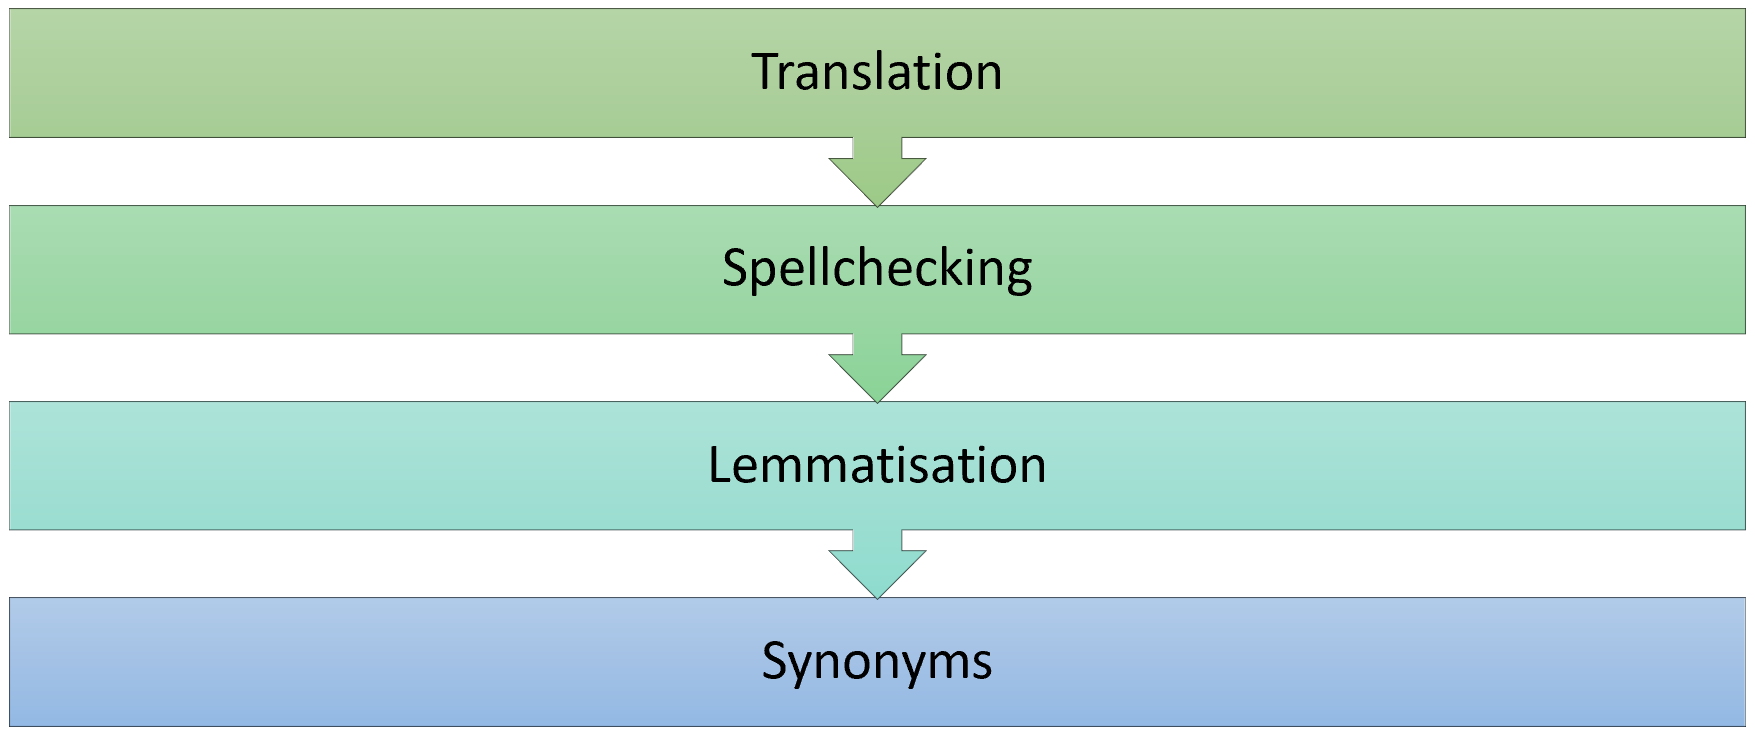
\includegraphics[width=\textwidth]{g14-semantics_pipeline.png}
	\caption{GUI for desktop screens}
	\label{fig:guiclassicdesktop}
\end{figure}



\subsubsection{Stemming}
\label{g14:sec:concepts:linguistics:stemming}
Words are reduced to their stems for counting, this allows user to use the inflection they deem appropriate. We do this with lemmatisation, which uses the part-of-speech of the word to reduce it to its stem instead of cutting of some letters.


\subsubsection{Synonyms}
\label{g14:sec:concepts:linguistics:synonyms}
For each tag synonyms are looked up and only the core word is added to the database. So for both 'big' and 'large' we would add 'large' as tag for this image.


\subsubsection{Translation}
\label{g14:sec:concepts:linguistics:translation}
The application has a set language and tags provided in other languages are translated to the set language.


\subsubsection{Phrasal Verbs}
\label{g14:sec:concepts:linguistics:phraselverbs}
The game accepts word combinations of up to two words to allow the use of phrasal verbs should the user provide them.

